\documentclass[11pt]{amsart}

\usepackage{macros-master}
%\usepackage{chngcntr}
%\counterwithout{equation}{section}

\begin{document}

\section*{September 16, 2022}

Today we will review material in sections 2.4--2.5 of the book.

Recall that we say
\beqn
\lim_{x \to a} f(x) = \infty
\eeqn
if we can make the value $f(x)$ be infinitely large by choosing $x$ to be sufficiently close to $a$.
Similarly, we can define 
\beqn
\lim_{x \to a} f(x) = \pm \infty , \quad \lim_{x \to a^{\pm}} f(x) = \pm \infty .
\eeqn
In any of these cases we call the line $x = a$ a vertical asymptote of the function $f$. 

\parsec
Challenge question. 
If $\lim_{x \to a} f(x) = \infty$ and $\lim_{x \to a} g(x) = - \infty$ then what can we say about $\lim_{x \to a} (f(x) + g(x))$? 

\vspace{5cm}

\begin{eg} 
Compute the following limit (if it exists)
\beqn
\lim_{x \to 0} \left(\frac{1}{x} - \frac{1}{x^2}\right) 
\eeqn
\end{eg}

\vspace{5cm}

\begin{eg}
Compute the following limit (if it exists)
\beqn
\lim_{x\to 0} \left(\frac{1}{x} - \frac{2x+1}{x}\right) .
\eeqn
\end{eg}
\newpage


\begin{eg}
Define the function
\beqn
f(x) = \frac{x^2-x-2}{x-a}
\eeqn
where $a$ is some number.
For which values of $a$ do the following limits exist.
\begin{itemize}
\item $\lim_{x\to a^+} f(x)$.
\item $\lim_{x \to a^-} f(x)$.
\item $\lim_{x\to a} f(x)$. 
\end{itemize}
\end{eg}

\newpage

\parsec[]

Recall that we say 
\beqn
\lim_{x \to \infty} f(x) = L
\eeqn
if we can make $f(x)$ as close to the value $L$ for $x$ a large enough number.
In this case we say that $y=L$ is a horizontal asymptote of the function $f$. 

\begin{eg}
Find the limit (if it exists)
\beqn
\lim_{x \to \infty}
\frac{x^2 + 2x + 1}{4x^2 + 5}
\eeqn
\end{eg}

\vspace{5cm}

\begin{eg}
Find the limit (if it exists). 
\beqn
\lim_{x \to \infty} \frac{e^x \sin x}{e^{2x} + 1}
\eeqn
\end{eg}

\newpage

\section*{September 19, 2022}

\begin{dfn}
Suppose that a function $f$ is defined on an open subset of $\R$ which contains the point $a$. 
We say that $f$ is continuous at $a$ if 
\beqn
f(a) = \lim_{x\to a} f(x) .
\eeqn
\end{dfn}

\parsec
Examples and non-examples of continuous functions .

\parsec 
Checklist for continuity.
For a function $f$ to be continuous at a point $a$, the following three conditions must hold.
\begin{enumerate}
\item $f$ must be defined at $a$.
\item the limit $L = \lim_{x \to a} f(x)$ must exist.
\item the limit $L$ must equal $f(a)$. 
\end{enumerate}

\begin{eg}
At which points $a \in \R$ is the function $f(x) = x / |x|$ continuous?
\end{eg}

\parsec
Properties of continuous functions. 
We say a function is continuous if it is continuous at all points in its domain. 
\begin{enumerate}
\item the sum, product, difference, and ratio (when defined) of two continuous functions is again continuous. 
\item all polynomials are continuous. 
\item Rational functions (ratios of polynomials) are continuous at every point in their domain. 
\item the composition of two continuous functions is again continuous. 
\end{enumerate}


\parsec 
Continuity on closed intervals. 
So far we've covered what it means for a function to be continuous on domains which are open intervals, like $(0,\infty)$. 
What about the function $f(x) = \sqrt{x}$ which is defined on the closed interval $[0,\infty)$? 
The problem is at the closed point $0 \in [0,\infty)$. 
In addition to checking continuity on the open interval $(0,\infty)$ we also need to make sure that the right sided limit at $0$ agrees with value of the function at that point
\beqn
\lim_{x \to 0^+} f(x) \overset{?}{=} f(0) .
\eeqn
If this is the case then we say that $f$ is continuous on the closed interval $[0,\infty)$. 

\newpage

\section*{September 22, 2022}

In the first week we defined the notion of average velocity which is the average rate of change of quantity position. 
We then motivated the definition of a limit by the idea of instantaneous rate of change.
In this lecture we return to the precise definition of the instantaneous rate of change of a function at a point---this is called the {\em derivative} of the function at a point. 

\begin{dfn}
The {\em derivative} of a function $f$ at a point $a$ is the limit
\[
f'(a) \define \lim_{x\to a} \frac{f(x) - f(a)}{x-a}
\]
when it exists. 
\end{dfn}

We say that $f$ is {\em differentiable} at $x=a$ if the derivative at $a$ exists. 
Otherwise we say that $f$ is not differentiable at $a$. 

\begin{eg} 
Using the limit definition above to compute the derivative of the function $f(x) = x^2 - 3x$ at the point $x = 1$. 
\end{eg}


\newpage


Graphically, the average rate of change of a function $y=f(x)$ on the interval $(a,a+\Delta x)$ is defined as 
\beqn
\frac{rise}{run} = \frac{\Delta y}{\Delta x} = \frac{f(a+\Delta x) - f(a)}{(a + \Delta x) - \Delta x} = \frac{f(a + \Delta x) - f(a)}{\Delta x} 
\eeqn 
We understood instantaneous rate of change of a function $y=f(x)$ as the limit 
\beqn
\frac{\Delta y}{\Delta x} \xto{\Delta x \to 0} f'(a)
\eeqn
Thus, the derivative at $x = a$ measures the {\em slope} of the graph at that point $(a, f(a))$.

\newpage

\section{September 23,2022}

Today we'll discuss more examples of derivatives. 

\subsection*{Examples}

\begin{eg}
Let 
\beqn
f(x) = \sqrt{x+7} .
\eeqn
\begin{itemize}
\item[(a)] Is the function $f(x)$ differentiable? If so, on what domain?
\item[(b)]
Use the limit definition to compute the derivative of $f(x)$ at $x=2$.
\item[(c)] 
Find the equation of the line tangent to the graph of the function $f(x)$ at $x=2$.
\end{itemize}
\end{eg}

\newpage

Here is an example of a function which fails to be differentiable at a point.

\begin{eg} Consider the absolute value function $f(x) = |x|$. 
At which point is $f(x)$ {\em not} differentiable. 
For the values of $x$ that $f(x)$ is differentiable, find $f'(x)$. 
\end{eg}

\vspace{3cm}

\subsection*{Properties of derivatives}

\begin{itemize}
\item (Constants) The derivative of a constant function $c(x) = c$ is identically zero, $c'(x) = 0$. 
If $c$ is any constant and $f$ is a function then
\beqn
(c f)' = c f' .
\eeqn
\item (Sum) The derivative of a sum is the sum of derivatives:
\beqn
(f+g)' = f' + g' .
\eeqn
\item (Power rule) For any integer $n$ the derivative of $f(x) = x^n$ is $f'(x) = n x^{n-1}$. 
In fact, if $r = p/q$ is a rational number then we still have
\beqn
(x^r)' = r x^{r-1} .
\eeqn
For example, the derivative of the function $\sqrt{x}$ is $1 / \sqrt{x}$.
\end{itemize}

\noindent \ul{\bf Warning}: The derivative of the {\em product} $f \cdot g$ is {\em not} the product of the derivatives:
\beqn
(f \cdot g)' \ne f' \cdot g'. 
\eeqn
Soon, we will learn rules for computing the derivative of the product of two functions. 

\newpage

\begin{eg}
Where is the function $f(x) = x^{2/3} + 7 x^{4}$ differentiable?
For the values of $x$ that $f$ is differentiable, what is $f'(x)$?
\end{eg}

\vspace{3cm}

\newpage

\section*{September 26, 2022}

\subsection*{Exponentials}

Today we continue with rules of derivatives, starting with the exponental function. 

\begin{dfn}
The exponential function $e^x$ is defined by
\beqn\label{eqn:exp}
e^x = \lim_{n \to \infty} \left(1 + \frac{x}{n}\right)^n
\eeqn
This number is defined for all real numbers $x$.
Approximately, one has 
\beqn
e \define e^1 = 2.71828\ldots .
\eeqn
\end{dfn}

The exponential function obeys the standard rules of exponentials.\footnote{Actually proving that $e^x = (e^1)^x$ is a good exercise.}
For instance, $e^0 = 1$.
Another good function to keep in mind is the natural logarithm which is the inverse to the exponential function:
\beqn
\ln(e^x) = e^{\ln x} = x 
\eeqn 
The natural logarithm $\ln x$ is only defined for $x > 0$.
A good limit to keep in mind is:
\beqn
\lim_{x \to \infty} e^x = \infty .
\eeqn

Let's turn to the derivative of the exponential function. 
First we have the following lemma.
\begin{lem}
One has
\[
\lim_{h \to 0} \frac{e^h - 1}{h} = 1.
\]
\end{lem}
\begin{proof}
Let's use equation \eqref{eqn:exp} to write 
\beqn\label{eqn:limith1}
\frac{e^h - 1}{h} = \frac{1}{h} \lim_{n \to \infty} \left(-1 + \left(1 + \frac{h}{n}\right)^n\right) .
\eeqn
Next, we use the binomial theorem to write
\begin{align*}
-1 + \left(1 + \frac{h}{n}\right)^n = -1 + \left(1 + n \frac{h}{n} + \cdots \right) = h + \cdots 
\end{align*}
where the $\cdots$ stands for terms which are at least quadratic in the parameter $h$. 
Plugging this back into \eqref{eqn:limith1} we obtain
\beqn
\frac{e^{h} - 1}{h} = 1 + \cdots
\eeqn
where now the $\cdots$ stands for terms that are at least linear in $h$. 
Taking the limit $h \to 0$ yields the result.
\end{proof}

\begin{eg}
Show that if $f(x) = e^x$ is the exponential function then
\beqn
f'(x) = e^x.
\eeqn
In other words the exponential is its own derivative $(e^x)'=e^x$.
This fact makes it very useful to model population growth, interest, etc. via the exponential function.
\end{eg}

\newpage

If $f = f(x)$ is a function, define the second derivative to be 
\beqn
f''(x) = (f'(x))' .
\eeqn
That is, this is the derivative of the derivative. 
Similarly we can define the third derivative $f'''(x)$, and so on. 

Recall that we have introduced the notation
\beqn
f'(x) = \frac{\d f}{\d x} .
\eeqn
We will also use
\beqn
f''(x) = \frac{\d^2 f}{\d x^2} 
\eeqn
and so on.

\begin{eg}
Let $f(x) = 3x^3 - 12 \sqrt{x}$.
Find $f''(x)$. 
\end{eg}

\vspace{3cm}

\begin{eg}
Find the twenty-first derivative of the function $f(x) = e^x - 3 x^{12}$. 
\end{eg}

\vspace{5cm}

\begin{eg}
Compute the limit 
\beqn
\lim_{a \to 1} \frac{\sqrt{3+a} - 2}{a-1}
\eeqn
(Hint: Don't compute the limit.)
\end{eg}

\newpage

\section{September 28, 2022}

Today we will cover the product and quotient rules for computing derivatives. 

Remember, the derivative $f' = \d f / \d x$ is motived by the concept of a `rate of change'. 
For average rate of change we wanted to consider how a function $f(x)$ changed as we change $x$ by some amount $\Delta x$:
\beqn
x \rightsquigarrow x + \Delta x .
\eeqn
When we change $x$ like this, the function $f(x)$ will then change like
\beqn
f(x) \rightsquigarrow f(x + \Delta x) = f (x) + \Delta f(x) 
\eeqn
where $\Delta f(x) = f(x+\Delta x) -f(x)$. 

We now want to consider what happens when we have a product of two functions $f \cdot g$. 
Then, we can think of $f \cdot g$ as changing like
\beqn
(f+\Delta f) \cdot (g + \Delta g) = f \cdot g + \Delta f \cdot g + f \cdot \Delta g + (\Delta f)\cdot (\Delta g) .
\eeqn
In calculus we study the instantaneous rate of change, which is the limit of the rate of change as the interval gets infinitesimally small.
So, we can imagine that the quantities $\Delta f$ and $\Delta g$ are extremely small. 
Then, if this is the case, we can think of the quantities $f \cdot \Delta g$ and $\Delta f \cdot g$ as being quite large as compared to $\Delta f \cdot \Delta g$.

In other words, we see that when $\Delta f$ and $\Delta g$ are very small, the amount that $f \cdot g$ changes by is approximately 
\[
\Delta f \cdot g + f \cdot \Delta g .
\]
This reasoning can be turned into the following theorem. 

\begin{thm}[Product rule]
Suppose that $f,g$ are differentiable functions. 
Then
\beqn
(f \cdot g)' = f' \cdot g + f \cdot g' .
\eeqn
\end{thm}

\begin{eg}
Using the power rule, ''check'' the product rule for the product of the two functions $f(x) = x^3$ and $g(x) = 5x^7$. 
\end{eg} 

\vspace{5cm}

\begin{eg} Compute the derivative of the function $f(x) = x^2 e^x$.
\end{eg}

\newpage

If $f,g$ are two differentiable functions and $g$ is nonzero (in some domain), then we can consider the derivative of the function $h = f/g$. 
Notice that we could also write this equation like $f = g \cdot h$. 
Applying the product rule we see that
\beqn
f' = g'\cdot h + g \cdot h' .
\eeqn
But, remember that we really wanted to know what $h'$ is.
For this, we can use the above equation to solve for this
\beqn
h' = \frac{f' - g' \cdot h}{g} = \frac{f' - g' \cdot f / h}{g} .
\eeqn
Rewriting this equation (in a completely equivalent way) results in the usual formulation of the quotient rule.

\begin{thm}[Quotient rule]
If $f,g$ are differentiable functions and $f/g$ is defined, then
\beqn
\left(\frac{f}{g}\right)' = \frac{f' g - f g'}{g^2} .
\eeqn
\end{thm}

\begin{eg}
Where is the following function differentiable?
\beqn
f(x) = \frac{x e^x}{1 + x^2} .
\eeqn
Compute the derivative of the function when it is defined.
\end{eg}

\vspace{8cm}

\begin{eg}
Compute the derivative of 
\beqn
f(x) = \frac{1-x^3}{1-x} .
\eeqn
Find the equation of the line tangent to the graph of $f(x)$ at $x = -1$. 
\end{eg}

\newpage

\section*{September 30, 2022}

Today we will discuss derivatives of trigonometric functions like
\beqn
\sin(x), \quad \cos(x), \quad \tan(x), \quad \text{etc} .
\eeqn

Recall the following limit
\beqn
\lim_{x \to 0} \frac{\sin x}{x} = 1 .
\eeqn
One nice proof of this uses some basic trigonometry for expressions of areas of triangles. 

\begin{eg}
What is the derivative of the function $\sin x$ at $x=0$? 
\end{eg}

\vspace{3cm} 

Another nice limit is the following 
\beqn
\lim_{x \to 0} \frac{\cos x - 1}{x} = 0 .
\eeqn
To obtain this notice that for $x \ne \pi,3 \pi, \ldots$ one has
\beqn
\frac{\cos x - 1}{x} = \frac{\cos x - 1}{x} \cdot \frac{\cos x + 1}{\cos x + 1} = \frac{\cos^2 x - 1}{x (\cos x + 1)} .
\eeqn
Now $\sin^2 x + \cos^2 x = 1$, so we can write this expression as 
\beqn
- \frac{\sin^2 x}{x (\cos x + 1)} = - \frac{\sin x}{x} \cdot \frac{\sin x}{\cos x + 1} .
\eeqn
Using the fact that the limit of the product of two functions is the product of the limits, we see that as $x \to 0$ this limit is $1 \cdot 0 = 0$. 

\begin{eg}
What is the derivative of the function $\cos x$ at $x = 0$? 
\end{eg}
\vspace{3cm}

Let's move on to general formulas for the derivatives of the functions $\sin x$ and $\cos x$. 

\begin{prop} 
One has
\beqn
(\sin x)' = \cos x, \qquad (\cos x)' = - \sin x .
\eeqn
\end{prop}
\begin{proof}
Let's consider just the derivative of $\sin x$. 
We appeal to a (hopefully familiar) trigonometric identity
\beqn
\sin(a + b) = \sin a \cos b + \cos a \sin b .
\eeqn
Now we compute
\begin{align*}
(\sin x)' & = \lim_{h \to 0} \frac{\sin(x+h) - \sin x}{h} \\
& = \lim_{h \to 0} \frac{\sin x \cos h + \cos x \sin h - \sin x}{h} \\ & = \sin x \cdot \left( \lim_{h \to 0} \frac{\cos h - 1}{h}\right) + \cos x \cdot \left(\lim_{h \to 0} \frac{\sin h}{h} \right) \\
& = \sin x \cdot 0 + \cos x \cdot 1 .
\end{align*} 
\end{proof}

\begin{eg}
Compute the derivative of the function 
\beqn
f(x) = e^x \cos(x) \sin (x) .
\eeqn
\end{eg}
\vspace{5 cm}

There are other trigonometric functions we can build using sine and cosine. 
For example, the tangent and cotangent functions are 
\beqn
\tan x = \frac{\sin x}{\cos x} , \quad \cot(x) = \frac{1}{\tan x} = \frac{\cos x}{\sin x} 
\eeqn 
And the secant and cosecant functions are 
\beqn
\sec x = \frac{1}{\cos x} , \quad \csc x = \frac{1}{\sin x} .
\eeqn

\begin{eg}
When is the function $\tan x$ well-defined? 
Use the quotient rule to compute the derivative 
\beqn
(\tan x)' .
\eeqn
Use this to find the equation of the line tangent to the graph $y = \tan x$ at the point $x = \pi / 4$. 
\end{eg}
 

\newpage

\section*{October 3, 2022}

Let's return to a real-world application of derivatives.
We've discussed that if $s(t)$ is the position of a particle as a function of time then the derivative $s'(t)$ represents the velocity as a function of time:
\beqn
s'(t) : \quad \text{velocity at time } t .
\eeqn
In other words, the rate of change of position is velocity. 

As we say last time, we can iterate the process of taking the derivative.
In other words, we can consider the second derivative $s''(t)$
This represents the rate of change of velocity as a function of time and is called the \textit{acceleration}. 

\begin{eg} 
Suppose a ball was thrown off of a cliff into the water at time $t=0$ and its height (in meters) above sea level (before hitting the water) is described by the following function if time (in seconds): 
\beqn
s(t) = 10 + 23 t - 5 t^2 .
\eeqn
At what time does the ball hit the water?
At what time is the ball moving the fastest? 
Describe the acceleration of the ball.
Can you determine the horizontal displacement of the ball?
\end{eg}

\newpage

\subsection*{Chain rule}

Now we will move onto the `chain rule'.
First, we need to remind ourselves how to compose functions. 
Given functions $f$ and $g$ such that the image of $g$ is contained inside the domain of $f$, the composition $h = f \circ g$ is defined.
One also write $h(x) = f (g(x))$. 

As an example, consider the functions $f(x) = x+1$ and $g(x) = \sqrt{x}$. 
Then 
\[
f (g(x)) = f(\sqrt{x}) = \sqrt{x} + 1 .
\]
Notice that the image of $g$ is the non-negative real numbers.
Since $f$ is defined everywhere, the function $f \circ g$ is defined wherever $g$ is defined, which is the non-negative real numbers.

In this example we can also consider the composition $g \circ f$ which is 
\[
g (f(x)) = g (x + 1) = \sqrt{x + 1} .
\]
Note here that the image of $f$ is all real numbers, so in order for the composition to be defined we must restrict $f$ to a smaller domain. 
In this example, the composition $g \circ f$ is defined whenever $x \geq -1$. 

\begin{eg}
Write the following functions as compositions of two functions
\beqn
e^{x^2}, \quad \sqrt{\sin(x) + 3}, \quad \sin(x^2) .
\eeqn
\end{eg}

\vspace{3cm}

The chain rule is a result which expresses the derivative of a composition of two functions $f \circ g$ in terms of the derivatives of the original two functions $f$ and $g$.

\begin{thm}
Suppose that $f,g$ are differentiable functions and that the composition is well-defined. 
Then $f \circ g$ is differentiable and 
\beqn
(f \circ g)' (x) = f'(g(x)) \cdot g'(x) .
\eeqn 
\end{thm}

Sometimes it is useful to introduce more variables.
Write $y = g(x)$ so that in this expression $x$ is the independent variable and $y$ is the dependent variable. 
On the other hand, we write $u = f(y)$ so that in this expression $y$ is the independent variable and $u$ is the dependent variable. 
Since $y$ depends on $x$ and $u$ depends on $y$, we see that $u$ depends on $x$.

Using this notation, we sometimes write derivatives as 
\[
f' = \frac{\d u}{\d y} , \quad g' = \frac{\d y}{\d x} .
\]
Then, heuristically we can view the chain rule as the following formula
\beqn
\frac{\d u}{\d x} = \frac{\d u}{\d y} \frac{\d y}{\d x} .
\eeqn

\newpage

\begin{eg} Find the derivative of 
\beqn
h(x) = \sqrt{e^x +1} .
\eeqn

\vspace{1cm}

Here we write $y = g(x) = e^{x} + 1$ and $f(y) = \sqrt{y}$. 
Then $h(x) = f(g(x))$. 
We compute $g'(x) = e^x$ and $f'(y) = \frac{1}{2 \sqrt{y}}$ so that via the chain rule
\beqn
h'(x) = f'(g(x)) g'(x) = \frac{e^x}{2 \sqrt{e^x + 1}}.
\eeqn 
\end{eg}

\newpage

\section*{October 5, 2022}

Today we will continue with more examples involving the chain rule.
Recall that the chain rule says that if $h = f \circ g$ is a composition of two functions then
\beqn
h'(x) = f'(g(x)) \cdot g'(x) .
\eeqn  

\begin{eg}
A function $f(x)$ is {\em even} if $f(-x) = f(x)$ and is {\em odd} if $f(-x) = -f(x)$. 
\begin{itemize} 
\item If $f$ is even, is the derivative $f'$ even, odd, or neither? 
\item If $f$ is odd, is the derivative $f'$ even, odd, or neither? 
\end{itemize} 
\end{eg}

\vspace{3cm} 

\begin{eg}
Express the function
\beqn
h(x) = \frac{1}{(2 x^2 + 3)^{10}} 
\eeqn
as a composition of two functions. 
Compute $h'(x)$ using chain rule.
\end{eg}

\vspace{5cm}

Let's see an example of chain rule where we do not necessarily know the exact form of one of the functions involved. 

\begin{eg}
Suppose that $f$ is differentiable and satisfies $f'(0) = 2$, $f'(1/2)=1/3$.
Let
\beqn
h(x) = f(\sin x) .
\eeqn
Find $h'(0)$ and $h'(\pi/6)$.
\end{eg} 

\newpage

\begin{eg} 
Let
\beqn
h(x) = x \sqrt{5-x^2} .
\eeqn
\begin{itemize} 
\item[(a)] Find $h'(x)$. 
\item[(b)] Determine the equation of the lines tangent to the graph at the values $x=1$ and $x=-2$.
\item[(c)] At which points (if any) do the lines in part (b) intersect? Express your answer as an ordered pair. 
\end{itemize} 
\end{eg} 


\newpage

Also, chain rule can be used to find limits. 

\begin{eg} 
Find the following limit (if it exists)
\beqn
\lim_{h \to 0} \frac{\sqrt{4 + \sin (h)} - 2}{h} .
\eeqn
\end{eg} 


\newpage

\section*{October 7, 2022}

Up until this point we have mostly been studying functions which are defined explicitly $y = f(x)$. 
Sometimes, in practical situations, we are know that a variable $y$ depends on a variable $x$, but the exact dependence is determined {\em implicitly}. 
For example, we can study an equation of the form 
\beqn
x^2 + y^2 = 1 .
\eeqn
In this plane, this equation represents the circle. 
On the other hand, if we think about $x$ as the independent variable, this equation does not determine a function $y = f(x)$ in a unique way.
In general, we would need some more information to determine $y$ as a function of $x$ (in this example, assuming that $y$ is non-negative is enough). 
In this situation, we say that $y$ depends {\em implicitly} on $x$.

Even if variables depend implicitly on each other, we can still ask for rates of change of one variable with respect to the other variable. 
Let's think about the example and ask about the derivative $\d y / \d x$. 

The first step is to think about $y=y(x)$ depending on $x$. 
Then the equation is 
\beqn
x^2 + (y(x))^2  = 1.
\eeqn
We then take the derivative of both sides with respect to $x$:
\beqn
\frac{\d}{\d x} \left(x^2 + y(x)^2\right) = \frac{\d}{\d x} (1) .
\eeqn
The right hand side is zero.
The left hand side is
\beqn
2 x + 2 y(x) y'(x) = 2 x + 2 y(x) \frac{\d y}{\d x} 
\eeqn
as we can see by applying the chain rule. 
Thus, the derivative of the equation is
\beqn
x + y(x) y'(x) = 0 .
\eeqn

Next, we solve for the derivative
\beqn
y'(x) = - \frac{x}{y(x)}.
\eeqn
as long as $y(x) \ne 0$. 
What is happening when $y = 0$? 

\begin{eg}
What are the slopes of the line tangents to the circle at $x = \frac12$. 
\end{eg}

\newpage

\begin{eg} 
Suppose that the variables $x,y$ satisfy 
\beqn
x^2 + y^3 = 1 .
\eeqn
Find $\frac{\d^2 y}{\d x^2}$. 
\end{eg}

\vspace{6cm} 

\begin{eg}
Find the equations for the vertical and horizontal tangent lines to the graph described by the following equation
\beqn
x^2 + 2 y^2 = xy .
\eeqn
\end{eg}

\newpage

\section*{October 11, 2022} 

Let's begin with one more example related to implicit derivatives. 

\begin{eg} 
Find equations for lines tangent to the graph
\beqn
y^2 - 3xy = 2
\eeqn
when $x = 1/3$. 
\end{eg}

\vspace{5cm} 

Next, we will move onto derivatives of logarithms. 
The natural logarithm $\ln x$ is, by definition, the inverse to the exponential function $e^x$. 
Recall that two functions $f(x), g(x)$ are said to be inverses of one another if 
\beqn
f(g(x)) = x, \quad \text{and} \quad g (f (x) ) = x. 
\eeqn 
Thus, the defining properties of the natural logarithm are
\beqn
\label{eqn:log1}
e^{\ln x} = x, \quad \text{and} \quad \ln e^x = x .
\eeqn
Some key identities to keep in mind when working with logarithms include $\ln(ab) = \ln a + \ln b$ and $\ln (a^r) = r \ln a$. 

Just the knowledge of the properties in \eqref{eqn:log1} will allow us to nail down the derivative of $\ln x$ using the rules that we know. 
First, introduce a dependent variable $y = \ln x$ into the first expression above:
\beqn
e^y = x .
\eeqn
Next, we take the implicit derivative with respect to $x$ to get
\beqn
e^y y' = 1 .
\eeqn
In other words, $y' = e^{-y}$. 
Substituting $y = \ln x$ we then obtain an explicit expression for the derivative.

\begin{prop}[Derivative of natural log] 
\beqn
\left(\ln x\right)' = e^{- \ln x} = \frac{1}{x} .
\eeqn
\end{prop}

\begin{eg}
Use the second expression in \eqref{eqn:log1} to `rederive' the formula $(e^x)' = e^x$. 
\end{eg}

\vspace{3cm} 

The expression $\ln x$ is only defined for $x > 0$. 
On the other hand, the expression $\ln |x|$ is defined for any $x \ne 0$. 

\begin{eg}
Use the chain rule to show that for all $x \ne 0$ one has 
\beqn
\left(\ln |x|\right)' = \frac{1}{x}.
\eeqn
\end{eg} 

\vspace{3cm}

\begin{eg}
Compute the derivative of $\ln \left(\sqrt{x+1}\right)$ in two ways.
\end{eg}

A simple application of chain rule shows the following. 

\begin{prop}
Suppose that $f$ is differentiable and $\ln (f(x))$ exists. 
Then
\beqn
\left(\ln (f(x))\right)' = \frac{f'(x)}{f(x)} .
\eeqn
\end{prop} 

Next, we consider functions which are like exponentials but where we use a different base. 
For example, consider the function $f(x) = 2^x$.
To compute the derivative we introduce the dependent variable $y = 2^x$ and write this expression as 
\beqn
y = 2^x \leftrightarrow \ln y = \ln (2^x) = x \ln 2 .
\eeqn
Thus, the original equation $y = 2^x$ is equivalent to the implicit representation 
\beqn
\ln y = x \ln 2 .
\eeqn
We then apply the derivative to get
\beqn
\frac{y'}{y} = \ln 2 .
\eeqn
In other words $y' = y \ln 2 = 2^x \ln 2$, so that
\beqn
\left(2^x\right)' = 2^x \ln 2 .
\eeqn

Without much more difficulty one can show. 
\begin{prop}
For $0 < b$ and $b \ne 1$ one has 
\beqn
\left(b^x\right)' = b^x \ln b .
\eeqn
\end{prop} 

\begin{eg}
Find the slope of the line tangent to the graph of $f(x) = x^{x}$ at $x=1$. 
Does this graph have any horizontal tangent lines? 
\end{eg} 

\newpage 

\section*{Practice for midterm 1}

The following list is a non-exhaustive of problems on material that we have covered so far. 
Don't expect to have time to complete all of these problems, this is just meant to be a large source of practice problems in case you run out of other material to prepare with. 

\begin{itemize}
\item \S 2.2, 18.
\item \S 2.3, 19-70, 72, 73.
\item \S 2.4, 8, 9, 21-44.
\item \S 2.5, 17-50.
\item \S 2.6, 17-20.
\item \S 3.1, 33-42. 
\item \S 3.2, 21-30, 35-40.
\item \S 3.3, 19-40.
\item \S 3.4, 19-60, 61-64, 76-81.
\item \S 3.5, 23-50. 
\item \S 3.6, 21-30. 
\item \S 3.7, 15-24, 26-76.
\item \S 3.8, 13-40.
\item \S 3.9, 15-48.
\item \S 3.10, 13-22. 
\item \S 3.11, 23-30, 42.
\end{itemize}

\newpage

\section*{October 24, 2022}

Let's begin with an exercise about extrema. 

\begin{eg} Find the absolute extrema for the function 
\beqn
f(x) = \frac{2x}{1 + x^2} 
\eeqn
on the interval $[-2,2]$. 
\end{eg} 

\vspace{5cm} 

The {\bf mean value theorem} is one of the most important theorems in calculus. 
It's the main player behind much of the techniques we will learn in the upcoming weeks about describing the behavior of functions. 

An easy case of the mean value theorem is Rolle's theorem. 
Consider a function $f$ which is continuous on a closed interval $[a,b]$ and differentiable on the open interval $(a,b)$.
Suppose, in addition, the function satisfies $f(a) = f(b)$. 
In this situation, we can conclude that there is at least one point $c$ with $a < c < b$ such that $f'(c) = 0$. 

\begin{eg}
Can you give a visual proof of this result? 
Consider the function $f(x) = 1 - x^2$ defined on the interval $[-1,1]$. 
\end{eg} 


The mean value theorem is just a skew, or rotated version, of Rolle's theorem. 
Suppose we take away the condition that $f(a) = f(b)$. 
We can still consider the average rate of change of the function $f$ on the interval $[a,b]$:
\beqn
\frac{f(a) - f(b)}{a-b} .
\eeqn
Remember, this quantity represents the average slope of tangent lines to the function on the interval. 

\begin{thm}
Consider a function $f$ which is continuous on a closed interval $[a,b]$ and differentiable on the open interval $(a,b)$.
Then, there exists a number $c$ with $a < c < b$ such that
\beqn
f'(c) = \frac{f(a) - f(b)}{a-b} .
\eeqn
\end{thm}


\begin{eg} 
Check the mean value theorem for the function $f(x) = x + \frac{1}{x}$ on the interval $[1,3]$. 
That is, find the number $c$ which is guaranteed by the mean value theorem. 
\end{eg}

\vspace{5cm} 

A nice corollary of the mean value theorem is the following. 

\begin{cor} 
Suppose that $f'(x) = 0$ for all $x$. 
Then $f$ is a constant function. 
\end{cor} 
\begin{proof} 
Let $a < b$ be two numbers. 
By the mean value theorem, there exists a $c$ with $a < c < b$ with the property that
\beqn
f'(c) = \frac{f(a)-f(b)}{a-b} .
\eeqn
But $f'(c) = 0$ by assumption, therefore $f(a) = f(b)$. 
\end{proof}

\newpage

\begin{eg} 
This problem involves calculus. 
\begin{itemize}
\item Show that $\arctan x$ and $\arctan (1/x)$ differ by a constant. 
\item Show that $\arctan x + \arctan(1/x) = \pi/2$ for $x > 0$. 
\end{itemize} 
\end{eg} 

\newpage 

Let $f(x) = \arctan x + \arctan 1/x$ and consider it on the domain $x > 0$. 
Then, 
\beqn
f'(x) = \frac1{1+x^2} + \frac{-1/x^2}{1+(1/x)^2} = \frac{1}{1+x^2} - \frac{1}{1+x^2} = 0.
\eeqn
Thus, by the corollary above we conclude that $f(x) = K$ for some constant $K$ for all $x > 0$. 
Similarly, we can show that $f(x) = K'$ for some constant $K'$ and all $x < 0$. 

Take $x = 1$, then we see
\beqn
K = f(1) = \pi/4 + \pi/4 = \pi/2 .
\eeqn 

\newpage

\section*{October 28, 2022} 

\begin{eg} 
Suppose that $f(x)$ is defined and differentiable everywhere. 
If $f'(x) > 0$ for all $x$ is it true that 
\beqn
\lim_{x \to \infty} f(x) = \infty ?
\eeqn
If not, try to find a counterexample. 
\end{eg} 

\vspace{5cm} 

Last time we covered the first derivative test.
Let's do an example. 
\begin{eg} 
Find the local and absolute extrema of the function 
\beqn
f(x) = \frac{x^2}{1-x^2} 
\eeqn
\end{eg} 

\newpage 

\begin{eg} 
Find the local and absolute extrema of the function
\beqn
f(x) = x^x
\eeqn 
defined for $x > 0$. 
\end{eg} 
\vspace{5cm} 

\newpage

\section*{October 31, 2022}

We've learned what the derivative tells us about the shape of a graph. 
What about the second derivative? 
This controls the feature called {\em concavity.}

\begin{itemize} 
\item A function is {\bf concave up} on an interval if $f'(x)$ is increasing on the interval. 
\item A function is {\bf concave down} on an interval if $f'(x)$ is decreasing on the interval. 
\item A point $x = c$ where $f$ changes concavity is called an {\bf inflection point.}
\end{itemize} 

An easy reformulation of the first two points is the following:

\begin{itemize}
\item If $f''(x) > 0$ on some interval, we say that $f$ is concave up on that interval. 
\item If $f''(x) < 0$ on some interval, we say that $f$ is concave down on that interval.
\item If $f''(c) = 0$ and $f''(c)$ changes sign as we go through $x=c$ then $x=c$ is an inflection point of the function. 
\end{itemize} 

\begin{eg}
Describe the concavity and the inflection points of the following functions.
\begin{itemize}
\item[(a)] $f(x) = \arctan(x)$.
\item[(b)] $f(x) = \sqrt{x} \ln x$ on the domain $x > 0$.
\end{itemize}
\end{eg}

\newpage

Next we move on to the second derivative test. 

Suppose that $x=c$ is a critical point of a function $f$ which satisfies $f'(c) = 0$. 
\begin{itemize} 
\item If $f''(c) > 0$ then $f$ has a local minimum at $x=c$. 
\item If $f''(c) < 0$ then $f$ has a local maximum at $x=c$. 
\end{itemize}
If $f''(c) = 0$ then the test is inconclusive---the function may have a local min/max or neither. 

\newpage

\begin{eg}
Use the second derivative test to locate and characterize the local extrema of the function 
\beqn
f(x) = \frac{e^x}{x+1}
\eeqn
defined for $x \ne 1$.
\end{eg}

\newpage

\section*{November 2, 2022}

We have many techniques to finding local extrema. 
Here is one that can be used to locate absolute extrema.

Suppose that $f(x)$ is defined on an interval and has exactly one local extrema at $x = c$. 
\begin{itemize}
\item if it is a local maximum at $x=c$ then it is an absolute maximum. 
\item if it is a local minimum at $x=c$ then it is an absolute minimum. 
\end{itemize} 

\vspace{3 cm}

Let's turn to an example that ties in a lot of the concepts we've discussed.

\begin{eg}
Consider the polynomial $g(x) = x^2 - x + 1$. 
Using calculus, show that $g(x)$ has no (real) roots. 
\end{eg} 

\newpage

Notice that $\lim_{x \to \pm \infty} g(x) = \infty$. 
Next, we find the local extrema. 
We have
\beqn
g'(x) = 2x - 1 ,
\eeqn
so there is a critical point at $x = 1/2$. 
But, $g''(1/2) > 0$, thus $g(x)$ attains a local minimum at $x = 1/2$.
Since this is the only extrema, this is in fact an absolute minimum of the function. 

Now, notice that 
\beqn
g(1/2) = 1/4 - 1/2 + 1 > 0 .
\eeqn
Thus, $g(x)$ has no roots. 

\vspace{1cm}

Here is a more involved example that uses similar ideas.

\begin{eg} Consider the function $f(x) = x \ln x - \ln x - x$ defined for $x > 0$. 
How many roots does the function $f(x)$ have? 
(Hint: use calculus.)
\end{eg} 

\newpage  

Notice that 
\beqn
\lim_{x \to 0^+} f(x) = \infty 
\eeqn
and 
\beqn
\lim_{x \to \infty} f(x) = \infty .
\eeqn
Based on this, it is possible that $f$ could have zero, two, four, etc. roots.
That is, we know it has an even number of roots. 
Let's nail this down.

Let's determine if the function has any local extrema. 
The derivative of $f(x)$ is
\beqn
f'(x) = \ln x - \frac{1}{x} . 
\eeqn
Notice that 
\beqn
\lim_{x \to 0^+} f'(x) = - \infty 
\eeqn
and 
\beqn
\lim_{x \to \infty} f'(x) = \infty .
\eeqn
In particular we see that the derivative $f'(x)$ must have at least one zero.

Let's next compute the second derivative
\beqn
f''(x) = \frac{1}{x} + \frac{1}{x^2} .
\eeqn
Notice that this function is always positive. 
Thus, $f'(x)$ is increasing everywhere.
In particular, we see that there is a unique solution to $f'(x) = 0$, let's call it $x = c$. 
Sine $f''(c) > 0$ we see that $f$ has a local minimum (hence absolute minimum) at $x=c$. 

Shuffling terms around, we see that $c$ satisfies
\beqn
\ln(c) - \frac1c = 0.
\eeqn
Since $c > 0$, this is equivalent to $c \ln c - 1 = 0$. 
Thus
\beqn
f(c) = c \ln c - \ln c - c = 1 - \frac{1}{c} - c = \frac{1}{c} \left(-c^2 + c - 1 \right) .
\eeqn
We showed in the last example that $-c^2 + c - 1 < 0$ for all $c$. 
Thus $f(c) < 0$.

We conclude that $f(x)$ has two roots.

%For $0 < x < c$ the derivative satisfies $f' < 0$. 
%For $x > c$ the derivative  

\newpage

We move on to optimization problems which generally ask the following:
\begin{itemize}
\item \textit{What is the minimum or maximum value of a quantity subject to some class of constraints?}
\end{itemize} 

Here is an example. 
Suppose we have a rectangle of lengths $x$ and $y$.
Neither $x$ nor $y$ are fixed, but we do impose the constraint that
\beqn
x + y = 1 .
\eeqn
Then, for what values of $x,y$ is the area of the rectangle maximized and minimized? 

To solve this, we recall that the area is
\beqn
A = xy .
\eeqn
Notice that this is a function of two variables $x,y$. 
But, the constraint tells us how $x,y$ are related, namely $y = 1-x$. 
Plugging this in, we see that the area is a function only of $x$
\beqn
A(x) = x (1-x) = x - x^2 .
\eeqn

The critical points of $A(x)$ are ones where $A'(x) = 0$ which is the condition $1 - 2x = 0$. So there is only one critical point at $x = 1/2$.
Since $A''(1/2) = -2$ this critical point is an absolute maximum. 
Notice that for $x=1/2$ we have $y=1/2$ by the constraint.
This is a square, and the area is $A=1/4$. 

What about the absolute minimum. 
Naively, we would say that the function $A(x) = x - x^2$ has no absolute minimum. 
But we need to be careful since we are thinking of $x$ as a length, so we are only considering the function on the domain $x > 0$ and $x < 1$ (the last condition arises from the constraint and the fact that $y > 0$.) 
Thus, we still see that there is no absolute minimum (we can take $x$ to be closer and closer to zero or one and get a smaller and smaller area).

\newpage

\begin{eg}
Find the point on the curve $y = x^2$ that is closest to the point $(18,0)$. 
(Hint: You may use the following fact
\beqn
2 \cdot 2^3 + 2 - 18 = 0  \quad .)
\eeqn
\end{eg} 

\newpage

Recall the formula for the distance between $P_1=(x_1,y_1)$ and $P_2=(x_2,y_2)$
\beqn
d(P_1,P_2)^2 = (x_1 - x_2)^2 + (y_1-y_2)^2 .
\eeqn

A point on the curve $y=x^2$ is of the form $P_1 = (x,x^2)$. 
We want to minimize the distance to the point $P_2 = (18,0)$. 
As a function of $x$, the distance squared is
\beqn
D(x) = d(x)^2 = (x-18)^2 + (x^2)^2 = (x-18)^2 + x^4 .
\eeqn
The derivative of this distance squared is
\beqn
D'(x) = 2 (x-18) + 4 x^3 = 2(2x^3 + x - 18) .
\eeqn
We want to describe solutions to $D'(x) = 0$, so it suffices to look at the equation $2x^3+x-18=0$. 
One method is to observe that this can be factored like
\beqn
(x-2)(2x^2 + 4x + 9) = 0 
\eeqn
and hence the only solution is $x=2$. 

Thus the point $(2,4)$ is the closest point on the curve of $y=x^2$ to the point $(18,0)$.

\newpage

\section*{November 4, 2022}

Another optimization problem. 

\begin{eg} 
A fence that is 6 feet high is running parallel to a house and is 3 feet away from the house.
What is the minimum length of a ladder which clears the fence and touches the house? 
\end{eg} 

\newpage

Let's denote by $x$ the distance, in feet, from the base of the ladder to the fence. 
Then the length between the base of the ladder and the house is $x + 3$.
Let $y$ be the height from the top of the ladder to the ground.
Then, the length of the ladder $\ell$ can be computed as
\beqn
\ell^2 = (x+3)^2 + y^2 .
\eeqn

The quantities $x,y$ are related by the following geometric constraint.
Using similar triangles we see that we have
\beqn
\frac{y}{x+3} = \frac{6}{x} .
\eeqn
In other words, $y = \frac{6(x+3)}{x}.$

We can use this to express the length of the ladder just in terms of the quantity $x$
\beqn
\ell(x)^2 = (x+3)^2 + \frac{36}{x^2} (x+3)^2 = (x+3)^2 \left(1 + \frac{36}{x^2} \right) .
\eeqn
We want to minimize the function $L(x) = \ell(x)^2$.

The first derivative is
\begin{align*}
L'(x) & = 2 (x+3) \left(1 + \frac{36}{x^2} \right) + (x+3)^2 \left(-\frac{72}{x^3}\right) \\
 & = (x+3) \left(2 (1 + 36/x^2) - (x+3) (72/x^3) \right) \\
 & = (x+3) \left(2 + 72/x^2 - 72/x^3 - 216/x^3 \right) \\
 & = (x+3) \left(2 - 216/x^3\right) .
\end{align*}

We have potential critical points at $x=-3$ and $x = \sqrt[3]{108} = 3 \sqrt[3]{4}$.
The point $x=-3$ is not meaningful since $x>0$ represents a length. 
Therefore we have only one critical point!

By computing $L''(3 \sqrt[3]{4})>0$ (or using the first derivative test) we see that this is a local, hence absolute, minimum. 

\newpage

\section*{November 7, 2022}

If we zoom in, the line tangent to a graph of a smooth function closely approximates the original function. 
Assume that $f$ is smooth on an interval containing $x=a$. 
The slope of the line tangent to the curve $y=f(x)$ at the point $(a,f(a))$ is $f'(a)$.
The equation of a line  tangent to the graph at this point, in slope intercept form, is
\beqn
y - f(a) = f'(a)(x-a)
\eeqn
or
\beqn
y = f(a) + f'(a) (x-a) .
\eeqn

Let 
\beqn
L_a(x) = f(a) + f'(a) (x-a)
\eeqn
be the function describing this line.
Then, we say that that $L_a(x)$ is the linear approximation of $f(x)$ near $x=a$ and will often write
\beqn
f(x) \approx L(x)
\eeqn
for $x$ near $a$.

\begin{eg} 
Find the linear approximation for the function $f(x) = \ln x$ and use it to approximate $\ln(1.1)$. 
\end{eg}

\vspace{4cm}

\begin{eg}
Find the linear approximation of $f(x) = \tan^3 (x)$ and use it to approximate $\tan(11 \pi/40)$. 
(Notice that $11/40 \approx 1/4$.)
\end{eg}

\vspace{5cm} 

We are trying to approximate the value of the function $f(x)=\tan^3(x)$ near $x=\pi/4$. 
The derivative is
\beqn
f'(x) = 3 \tan^2(x) \sec^2(x) .
\eeqn
The line $y=L(x)$ tangent to the graph at $x=\pi/4$ is 
\beqn
L(x) - f(\pi/4) = f'(\pi/4) (x-\pi/4) .
\eeqn

Let's record the relevant values of the function and the derivative:
\beqn
f(\pi/4) = 1, \quad f'(\pi/4) = 3 \cdot 1 \cdot (\sqrt{2})^2 = 6 .
\eeqn
So plugging all of this in:
\beqn
L(x) = 6(x-\pi/4) + 1 .
\eeqn


\newpage

Let's move on to L'H\^{o}pital's rule. 
The most basic application of this rule is to compute limits of the following form
\beqn
\lim_{x \to a} \frac{f(x)}{g(x)}
\eeqn
where $f(a) = g(a) = 0$.

If $f,g$ are continuous and differentiable functions near $x=a$, we can use a linear approximation to compute either of the limits $\lim_{x \to a} f(x)$ or $\lim_{x\to a} g(x)$. 
Take $f(x)$ for example: near $x=a$ we have seen that $f(x)$ is approximated by the linear function
\beqn
L_f(x) = f(a) + f'(a) (x-a) .
\eeqn
Notice that 
\beqn
\lim_{x\to a} f(x) = \lim_{x \to a} L(x) = f(a) .
\eeqn
Similarly, there is a linear function 
\beqn
L_g(x) = g(a) + g'(a) (x-a) 
\eeqn
which approximates $g$ near $x=a$. 

We can attempt to use these approximations to compute the original limit $\lim_{x \to a} \frac{f(x)}{g(x)}.$
Indeed, near $x=a$ we have
\beqn
\frac{f(x)}{g(x)} \approx \frac{L_f(x)}{L_g(x)} = \frac{f(a) + f'(a) (x-a)}{g(a) + g'(a) (x-a)} .
\eeqn
But the assumption was that $g(a) = f(a) = 0$, so
\beqn
\frac{f(x)}{g(x)} \approx \frac{f'(a) (x-a)}{g'(a) (x-a)} .
\eeqn
Notice that for $x\ne a$ we have shown that 
\beqn
\frac{f(x)}{g(x)} \approx \frac{f'(a)}{g'(a)} 
\eeqn 

One can turn this into the following theorem. 

\begin{thm} 
Suppose that $f,g$ are differentiable on an interval containing $x=a$ and assume that $g'(x) \ne 0$ on this interval for $x \ne a$. 
Also, assume that $\lim_{x \to a}f(x) = \lim_{x \to a} g(x) = 0$. 
Then
\beqn
\lim_{x \to a} \frac{f(x)}{g(x)} = \lim_{x \to a} \frac{f'(x)}{g'(x)} .
\eeqn
\end{thm} 


\newpage

\section*{November 9, 2022}

We continue with L'H\^opital's rule. 
Recall that the first indeterminate form `0/0' that we can apply this rule to can be carefully stated as follows.

\begin{thm} 
Suppose that $f,g$ are differentiable on an interval containing $x=a$ and assume that $g'(x) \ne 0$ on this interval for $x \ne a$. 
Also, assume that $\lim_{x \to a}f(x) = \lim_{x \to a} g(x) = 0$. 
Then
\beqn
\lim_{x \to a} \frac{f(x)}{g(x)} = \lim_{x \to a} \frac{f'(x)}{g'(x)} .
\eeqn
\end{thm}

\begin{eg}
Evaluate the limit if it exists
\beqn
\lim_{x \to 0} \frac{e^x - 1}{\sqrt{x^3+1} - 1} .
\eeqn
\end{eg}


\vspace{2cm} 

Let's now consider the indeterminate form $\infty/\infty$. 

\begin{thm}
Suppose that $f,g$ are differentiable on an open interval containing $a$ with $g'(x) \ne 0$ for $x \ne a$ on this interval.
If $\lim_{x \to a} f(x) = \pm \infty$ and $\lim_{x\to a} g(x) = \pm \infty$, then
\beqn
\lim_{x \to a} \frac{f(x)}{g(x)} = \lim_{x \to a} \frac{f'(x)}{g'(x)} .
\eeqn
\end{thm}
Notice that this is the same conclusion as in the other indeterminate form $0/0$. 

We can use this to alternatively compute some familiar limits. 
\begin{eg}
Compute the limit using L'H\^opital's rule
\beqn
\lim_{x \to \infty} \frac{x^3 + 3}{2x^3 + x^2 +1}
\eeqn
\end{eg} 

\newpage 

Let's now move onto an example that isn't immediately in one of the indeterminate forms above. 

\begin{eg} 
Compute the limit if it exists
\beqn
\lim_{x \to 0^+} x \cdot \ln x .
\eeqn
\end{eg}

\vspace{2cm}

Notice that naively plugging in $0$ (or really a small positive number) we will get the indeterminate form $0 \cdot (-\infty)$. 
To do this example we rewrite the function as
\beqn
x \ln x = \frac{\ln x}{1/x} .
\eeqn
Note that now we have put this in the indeterminate form $-\infty/\infty$, so we can apply the rule.
\beqn
\lim_{x \to 0^+} x \cdot \ln x = \lim_{x\to 0^+} \frac{1/x}{-1/x^2} = -\lim_{x\to 0^+} x = 0 .
\eeqn


\newpage

\section*{November 11, 2022}

Last time we showed that 
\beqn
\lim_{x \to \infty} \frac{\ln x}{x} = 0 . 
\eeqn

This kind of limit suggests insight into the `growth rate' of functions. 
We say that a function $g$ {\bf grows faster} than a function $f$ if 
\beqn
\lim_{x \to \infty} \frac{f(x)}{g(x)} = 0 .
\eeqn
Equivalently, $\lim_{x \to \infty} g(x) / f(x) = \infty$. 
We say that the growth rates of $f,g$ are {\bf comparable} if the limit $\lim_{x \to \infty} f(x) / g(x)$ is a finite nonzero number.

\begin{eg}
In the last example, we saw that $x$ grows faster than $\ln x$. 
\end{eg}

\vspace{2cm}

\begin{eg}
\begin{itemize}
\item
Are there any $p,q > 0$ such that $(\ln x)^p$ and $x^q$ have comparable growth?
\item 
Are there any $p,q > 0$ such that $e^{px}$ and $x^q$ have comparable growth? 
\end{itemize}
\end{eg}

\newpage


\section*{November 14, 2022}

Given a differentiable function $g(x)$ we know we can consider its derivative $g'(x)$. 

\begin{itemize}
\item \ul{Question}: Given a function $f(x)$, does there exist a function differentiable function $F(x)$ such that 
\beqn
F'(x) = f(x) \quad ?
\eeqn
\end{itemize}

If we can find such a function $F(x)$ we call it an \textit{antiderivative} of $f(x)$. 

\begin{eg} 
What is an antiderivative of the function $f(x) = 1$? How about the function $f(x) = x$? 
In general, what is an antiderivative of $f(x) = x^n$?
\end{eg} 

\vspace{3cm} 

\begin{itemize}
\item \ul{Question}: How unique is an antiderivative? 
That is, if $F(x),G(x)$ are two antiderivatives of $f(x)$, then how close are $F(x)$ and $G(x)$ to being the same? 
\end{itemize}

\vspace{2cm}

\begin{thm} 
Suppose that $F(x),G(x)$ are two antiderivatives of $f(x)$. 
Then there exists a constant $C$ such that 
\beqn
F(x) = G(x) + C .
\eeqn
\end{thm}

\begin{proof}
We showed in the Mean Value Theorem section that if $f'(x) = g'(x)$ then $f (x)= g(x) + C$ for some constant $C$. 
Apply this to $f = F$ and $g=G$. 
\end{proof} 

\begin{eg} Find all antiderivatives of $\frac{1}{x}$. 
Next, find all antiderivatives of $\cos (2x)$. 
\end{eg} 

\vspace{2cm} 

\begin{eg} 
Are the following statements true? 
\begin{align*}
\left(\sin^2 x\right)' & = 2 \sin x \cos x \\
\left(-\cos^2 x\right)' & = 2 \sin x \cos x ?
\end{align*} 
If so, what does this say about the antiderivatives of $2 \sin x \cos x$? 
\end{eg}

\newpage

We will introduce the following symbol called the integral. 
We call 
\beqn
\int f(x) \d x
\eeqn
the {\em indefinite integral} of $f(x)$. 
It is meant to represent all possible antiderivatives of $f(x)$.
Thus, for example
\beqn
\int x \d x = \frac12 x^2 + C
\eeqn
where $C$ is an arbitrary constant.

\begin{itemize}
\item When we say `evaluate' $\int f(x) \d x$, we mean to find all possible antiderivatives of the function $f(x)$. 
\end{itemize}

\begin{eg}
Evaluate $\int \frac{\d x}{1 + x^2}$. 
How about $\int \frac{\d x}{2 + x^2}$? 
\end{eg}

\newpage

A (first-order) \textit{differential equation} is an equation of the form 
\beqn
f'(x) = g(x)
\eeqn
or if $y = f(x)$ this reads
\beqn
y' = g(x) .
\eeqn
A typical problem is to find solutions $y=f(x)$ to this equation. 
As we just saw this is no uniquely determined. 
But, if we impose some extra conditions then we can solve for $y=f(x)$ uniquely. 

\begin{eg}
Find the function $y = f(x)$ defined for $x > 0$ which solves the following equation 
\beqn
y' = 3x^2 + \sqrt{x} 
\eeqn
and satisfies $f(1) = 0$. 
\end{eg}
Such a problem is called an \textit{initial value problem}. 

\newpage

\section*{Practice for midterm 2}

The following list is a non-exhaustive of problems on material that we have covered (so far) that will be relevant for midterm 2.
Please note, midterm 2 will cover more material than what these problems indicate, please keep up-to-date on this list as we add more sections.
Don't expect to have time to complete all of these problems, this is just meant to be a large source of practice problems in case you run out of other material to prepare with. 

\begin{itemize}
\item \S 4.3 , 19--58, 77--94, 99. 
\item \S 4.5, 17--40, 51 (some of these are much harder than others). 
\item \S 4.6, 25--36. 
\item \S 4.7, 17--83, 95-98, 117. 
\item \S 4.9, 11--82. 
\item \S 5.1, 9,10, 17-22, 23-26, 32, 33, 37-40. 
\item \S 5.2, 39-46, 47-50
\end{itemize}

\newpage

\section*{November 16, 2022}

We have introduced integration as the formal inverse to the derivative. 
What is the geometric meaning of integration? 

Let's take an example. 
Suppose that the velocity of a car obeys 
\beqn
v(t) = 35 \quad \text{miles per hour}. 
\eeqn
To compute how far the car travels in 2 hours, we simply multiply
\beqn
35 \; \frac{\text{mi}}{\text{hr}} \times 2 \; \text{hr} = 70 \; \text{mi} .
\eeqn

Graphically, $v(t)$ is just a horizontal line. 
Geometrically, the quantity we just computed = distance traveled, represents the area of the rectangle of height $35$ and width $2$. 

More generally, if $v(t)$ was some interesting function of $t$ we arrive at the following hope / conjecture.

\begin{conj2}
The total distance traveled from time $t_0$ to time $t_1$ by a particle moving with velocity function $v(t)$ is represented by the area under the curve of $v(t)$ on the interval~$[t_0,t_1]$. 
\end{conj2}

To spoil the punchline, the area under the curve will be closely related to integration. 
For now, we will restrain ourselves to approximating areas under curves using rectangles. 
In some cases though, we can compute the area directly.

\vspace{2cm}

\begin{eg}
Consider the velocity function $v(t) = t$.
How far does the particle travel from time $t=0$ to time $t=2$?
(Hint: draw a picture.)
\end{eg}

\newpage

Let's consider a slightly more interesting example where a particle travels according the velocity function $v(t) = t^2$. 
We will approximate how far the particle travels from time $t=0$ to time $t=2$ using the following steps.

\begin{itemize}
\item[(1)] The first step is to divide the interval $[0,2]$ into smaller intervals. 
So, for example, we can divide it into four smaller intervals
\beqn
[0,2] = [0,1/2] \cup [1/2,1] \cup [1,3/2] \cup [3/2,2] 
\eeqn
(We will always assume that the sub-intervals are equal size).
\item[(2)] 
We then draw rectangles corresponding to each sub-interval whose top left corner touch the graph. 
So here we would draw four rectangles of width $1/2$ and of heights $v(0) = 0, v(1/2) = 1/4, v(1) = 1, v(3/2) = 9/4$, respectively. 
\item[(3)] To approximate the area we simply add up the areas of all rectangles.
In this case
\beqn
\text{Area} \approx \frac12 \cdot 0 + \frac12 \cdot \frac14 + \frac12 \cdot 1 + \frac12 \cdot 9/4 = \frac{7}{4} = 1.75.
\eeqn
\end{itemize}

\vspace{2cm}

The technical term for what we just computed was the {\bf left Riemmann sum approximation} to the area under the curve $v(t) = t^2$ between $t=0$ and $t=2$ using four subintervals. 

\begin{eg}
Approximate the same area using eight subintervals.
\end{eg}

\vspace{2cm}

\beqn
\text{Area} \approx \frac14 \cdot 0 + \frac14 \cdot \frac1{16} + \frac14 \cdot \frac14 + \frac14 \cdot \frac{9}{16} + \frac14 \cdot 1 + \frac14 \cdot \frac{25}{16} + \frac14 \cdot \frac94 + \frac14 \cdot \frac{49}{16} = \frac{425}{192} \approx 2.21
\eeqn


The actual answer is Area = $8/3 \approx 2.67$.
We're getting closer! 


\newpage

\section*{November 18, 2022}

Last time we introduced the left Riemann sum approximation to area under a curve. 
Let's now look at variants of this: the right and midpoint Riemann sums. 

The situation is that we have a function $y=f(x)$ defined on some interval $[a,b]$. 
The steps to approximate the area are as follows. 
\begin{itemize}
\item[(1)] Determine the number subintervals $n$ that we will partition the interval $[a,b]$ into.
The length of a subinterval is 
\beqn
\Delta x = \frac{b-a}{n} .
\eeqn
\item[(2)]
Draw $n$ rectangles as follows:
\begin{itemize}
\item In the {\bf left} Riemann sum, the top left corner of each rectangle touches the function. 
So you would draw $n$ rectangles of width $\Delta x$ and of heights 
\beqn
f(a), f(a+\Delta x), f(a + 2 \Delta x) , \ldots, f(a + (n-1) \Delta x) = f(b - \Delta x) .
\eeqn
\item In the {\bf right} Riemann sum, the top right corner of each rectangle touches the function.
So you would draw $n$ rectangles of width $\Delta x$ and of heights 
\beqn
f(a+\Delta x), f(a + 2 \Delta x) , f(a + 3 \Delta x), \ldots, f(a + n \Delta x) = f(b) .
\eeqn
\item In the {\bf midpoint} Riemann sum, the center of each rectangle touches the function. 
So you would draw $n$ rectangles of width $\Delta x$ and of heights 
\beqn
f(a + \frac12 \Delta x), f(a + \frac32 \Delta x), f(a + \frac52 \Delta x), \ldots, f(b-\frac12 \Delta x) .
\eeqn
\end{itemize} 
\item[(3)]
The last step is to sum the areas of the rectangles. 
\end{itemize}


\newpage

\begin{eg}\;

\begin{center}
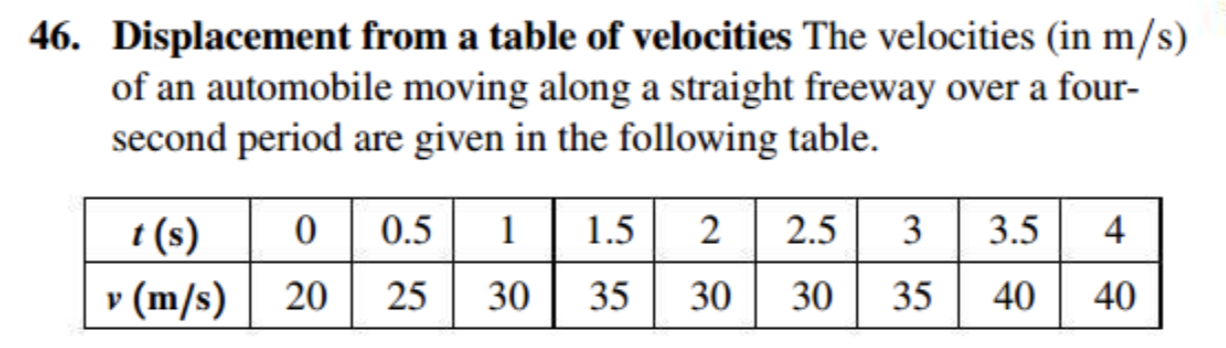
\includegraphics[scale=.5]{velocity}
\end{center} 

Use the midpoint Riemann sum approximation with four subintervals to approximate the distance traveled by the automobile from $t=0$ to $t=4$. 
\end{eg}

\newpage

\section*{November 21, 2022}

Last time we introduced the concept of {\em net area}. 
Let's recall the precise definition.

\begin{dfn}
Let $f$ be a continuous function and consider the region which is bounded by the $x$-axis and the curve of the graph $y=f(x)$ between $x=a$ and $x=b$. 
The {\em net area} is the area of the region above the $x$-axis minus the area below the $x$-axis.
\end{dfn} 

\vspace{1cm} 

\begin{eg} 
Consider the function $f(x) = 2x - 2$. 
What is the net area determined by $y = f(x)$ between $x=0$ and $x=2$?
What about the net area between $x=0$ and $x=3$? 
(Use geometry to obtain the {\em exact} answer, do not use a Riemann sum approximation.)
\end{eg}

\vspace{2cm} 

\begin{dfn}
Consider a function $f$ defined on an interval $[a,b]$ 
The {\em definite integral} (if it exists) 
\beqn
\int_{a}^b f(x) \d x 
\eeqn
is the net area determined by $y = f(x)$ between $x=a$ and $x=b$. 
\end{dfn} 

\begin{rmk}
This is actually more of a theorem than a definition, but the definition of the definite integral is a little more involved than what we will be focusing on in this class. 
We'll give a more precise definition in terms of Riemann sums at the end of this lecture.
\end{rmk} 

The existence is guaranteed in two situations.
\begin{itemize}
\item the function $f$ is continuous on the interval $[a,b]$, or 
\item the function $f$ is bounded with only finitely many discontinuities.
\end{itemize} 

\vspace{1cm} 

\begin{eg} 
Consider the function $f(x) = \sqrt{9 - x^2}$. 
Use geometry to compute
\beqn
\int_0^3 \sqrt{9-x^2} \, \d x .
\eeqn
\end{eg}

\newpage 

\begin{eg} 
Using geometry evaluate 
\beqn
\int_{-2}^4 \sqrt{8 + 2x - x^2} \, \d x .
\eeqn
\end{eg}

\vspace{4cm} 

\begin{eg} 
This example is about definite integrals of even and odd functions. 
\begin{itemize}
\item 
Suppose that $f(x)$ is an {\em even} function and $\int_0^2 f(x) \d x = 7$. 
Evaluate 
\beqn
\int_{-2}^2 f(x) \, \d x.
\eeqn
\item Suppose that $g(x)$ is an {\em odd} function. 
Evaluate
\beqn
\int_{-2}^2 g(x) \, \d x .
\eeqn
\end{itemize}
In general, what can you infer about integrals of even/odd functions around intervals that are symmetric about the $y$-axis? 
\end{eg} 

\newpage

Let's turn to a precise definition of the definite integral which uses Riemann sums. 
Recall that the Riemann sum approximating the net area of a function $f$ between $x=a$ and $x=b$ can be written as 
\beqn
f(x_1^*) \cdot \Delta x + f(x_2^*) \Delta x + \cdots + f(x_n^*) \Delta x 
\eeqn
where
\begin{itemize}
\item $n$ is the number of rectangles/subintervals.
\item $\Delta x = (b-a)/n$.
\item $x_k^*$ is either the left/midpoint/right point of the $k$th subinterval depending on the type of Riemann sum we use. 
\end{itemize} 
We can write this in a compact form using ``sigma-notation''
\beqn
\sum_{k=1}^n f(x_k^*) \Delta x .
\eeqn

More generally sigma-notation is simply shorthand for expressing a sum of numbers
\beqn
\sum_{k=1}^n g(k) = g(1) + g(2) + \cdots + g(n-1) + g(n) .
\eeqn
There are $n$ terms on the right hand side. 
\begin{eg}
Evaluate the sum $\sum_{k=1}^3 k^2$. 
\end{eg} 

More generally, there is a formula for this sum
\beqn
\sum_{k=1}^n k^2 = \frac{n(n+1)(2n+1)}{6} .
\eeqn
(If you like you can check this for small values of $n$.)

\vspace{1cm} 

We can now make this idea precise that Riemann sums approximate areas. 
\begin{dfn} 
The definite integral of $f$ from $x=a$ to $x=b$ (if it exists) is the limit of a Riemann sum approximation as the number of subintervals $n$ approaches $\infty$.
That is
\beqn
\int_a^b f(x) \d x = \lim_{n \to \infty} \sum_{k=1}^n f(x_k^*) \Delta x .
\eeqn
\end{dfn}

\newpage

\begin{eg} 
Let's evaluate $\int_1^2 x^2 \d x$ using the definition. 
\end{eg} 

We will use the left Riemann sum approximation. 
For instance, when $n = 4$ we have $\Delta x = 1/4$ and the left Riemann sum is
\beqn
1^2 \cdot \frac14 + \left(\frac54\right)^2 \cdot \frac14 + \left(\frac{3}{2}\right)^2 \cdot \frac14 + \left(\frac{7}{4}\right)^2 \cdot \frac14 .
\eeqn

For general $n$ we have the Riemann sum approximation
\begin{align*}
\sum_{k=1}^n \left(1+\frac{k}{n}\right)^2 \frac1n & = \sum_{k=1}^n \frac{(n+k)^2}{n^3} \\ & = \sum_{k=1}^n \left(\frac{1}{n} + \frac{2k}{n^2} + \frac{k^2}{n^3} \right) \\ &= 1 + \frac{n+1}{n} + \frac{n(n+1)(2n+1)}{6n^3} .
\end{align*} 

Taking $n \to \infty$ we obtain
\beqn
1 + 1 + \frac13 = \frac73 .
\eeqn
 
\newpage

\section*{November 28, 2022}

We've introduced the definite integral 
\beqn
\int_a^b f(t) \, \d t
\eeqn
as the net area under between the graph $y=f(t)$ and the $t$-axis between $t=a$ to $t=b$. 
A precise definition was given in terms of a limit of Riemann sums. 

Let's imagine fixing a function $f(t)$ and a starting point $t=a$ of some interval. 
Then, we can express the net area between the graph $y=f(t)$ and the $t$-axis between $t=a$ and some variable number $t=x$ as 
\beqn
N(x) = \int_a^x f(t) \, \d t .
\eeqn
Notice that $N$ is a function of $x$ and {\bf not a function of} the ``dummy'' variable $t$.

\begin{eg}
Find the area function $N(x)$ determined by the function $f(t) = t$ and the number $a=-1$. 
Is $N(x)$ a differentiable function? If so, compare the derivative $A'$ to the original function $f$.
\end{eg}

\newpage

The example above is a simple illustration of a important theorem.

\begin{thm}[The fundamental theorem of calculus]
Let $N(x) = \int_a^x f(t) \d t$ be the area function of the function $f$. 
Assume that $f$ is continuous on the interval $[a,b]$. 
Then $N(x)$ is continuous on the interval $[a,b]$ {\em and} differentiable on the interval $(a,b)$. 
Furthermore
\beqn
N'(x) = f(x)
\eeqn
on this interval. 
In particular, $N(x)$ is an antiderivative for $f(x)$ on the interval $[a,b]$.
\end{thm} 

\vspace{2cm}

Here is a sketch of the proof. 
Let's look at small sub interval $[x,x+h]$ where $h$ is a small number.
The area between the graph $y=f(t)$ on this interval is 
\beqn
N(x+h) - N(x) .
\eeqn
If we assume that $f$ is approximately constant on this interval, then this quantity is approximately the area of a rectangle
\beqn
N(x+h) - N(x) \approx h f(x) .
\eeqn
Or, dividing by $h$ we have
\beqn
\frac{N(x+h) - N(x)}{h} \approx f(x) .
\eeqn

This line of reasoning can be turned into a proof that 
\beqn
N'(x) = \lim_{h \to 0} \frac{N(x+h) - N(x)}{h} = f(x) .
\eeqn

\newpage

Because $N(x)$ is an antiderivative for $f(x)$ we know that any other antiderivative $F(x)$ of $f(x)$ differs by a constant
\beqn
F(x) = N(x) + C .
\eeqn
Of course, $N(a) = 0$, so that $C = F(a)$.
In particular we obtain the following important corollary.

\begin{cor}
Suppose $f$ is continuous on the interval $[a,b]$ and that $F(x)$ is an antiderivative for $f$ on this interval.
Then $N(b) = F(b) - F(a)$---equivalently, we have
\beqn
\int_a^b f(x) \, \d x = F(b) - F(a) .
\eeqn
\end{cor}

\vspace{2cm}

It will be useful to introduce the following notation
\beqn
F(x)|_a^b = F(b) - F(a) ,
\eeqn 
so that the above result can be written as 
\beqn
\int_a^b f(x) \d x = F(x)|_a^b .
\eeqn

\newpage

\section*{November 30, 2022} 

Last time we reviewed the most important theorem in calculus. 
The fundamental theorem states that if $f$ is a continuous function then
\beqn
N'(x) = f(x) 
\eeqn
where $N(x) = \int_a^x f(x) \d x$ is the net area function corresponding to $f$.
Equivalently, this can be written as
\beqn
\frac{\d}{\d x} \int_a^x f(x) \d x = f(x) .
\eeqn

As a consequence, $N(x) = \int_a^x f(x) \d x$ is an antiderivative of the function $f$. 
From this we deduce that if $F = \int f(x) \d x$ (this is the indefinite integral symbol) is any other antiderivative of $f$ then
\beqn
\int_a^b f(x) \d x = F(b) - F(a) \define F(x)|_a^b.
\eeqn

\vspace{1cm} 

\begin{eg} Evaluate 
\beqn
\int_0^3 e^{2x} \d x .
\eeqn
\end{eg} 

\vspace{3cm}

\begin{eg} Evaluate 
\beqn
\int_0^1 \frac{1}{3+3x^2} \d x . 
\eeqn
\end{eg}

\newpage

It's a good time to study some properties of the definite integral. 

$\bullet$ For any continuous function $f$ and $a$ any number, one has
\beqn
\int_a^a f(x) \d x = 0 .
\eeqn
This is because the net area is clearly zero as the width of the interval is null.

$\bullet$ For any continuous function $f$ and numbers $a < b < c$ one has
\beqn
\int_a^c f(x) \d x = \int_a^b f(x) \d x + \int_b^c f(x) \d x .
\eeqn
Geometrically this is just partitioning the region of integration into two smaller regions. 

One thing we've sort of taken for granted is that $\int_a^b f(x) \d x$ is defined when $a<b$ (using the definition in terms of net area). 
It's easy to extend this more generally.

$\bullet$ For any continuous function $f$ an numbers $a<b$ one has 
\beqn
\int_b^a f(x) \d x = - \int_a^b f(x) \d x .
\eeqn
One can take this as a definition.

$\bullet$ For any two functions $f,g$ one has 
\beqn
\int_a^b ( f(x) + g(x) ) \d x = \int_a^b f(x) \d x + \int_a^b g(x) \d x .
\eeqn

$\bullet$ For any constant $c$ one has 
\beqn 
\int_a^b c f(x) \d x = c \int_a^b f(x) \d x.
\eeqn

\begin{eg}
Compute 
\beqn
\int_1^2 (x^2 + 3x - 1) \d x 
\eeqn
\end{eg}

\newpage

Let's give a formal proof of the fundamental theorem. 
Let $N(x) \int_a^x f(x) \d x$ be the net area function, then its derivative, by definition, is 
\beqn
N'(x) = \lim_{h \to 0} \frac{N(x+h) - N(x)}{h} .
\eeqn

Using formal properties of integrals we have the following relation
\beqn\label{eqn:differenceftc}
N(x+h) - N(x) = \int_a^{x+h} f(x) \d x - \int_a^x f(x) \d x = \int_x^{x+h} f(x) \d x .
\eeqn

Let $m(x),M(x)$ be the minimum and maximum values of $f$ on the small interval $[x,x+h]$. 
(These exist by the extreme value theorem.)
Then 
\beqn
m(x) \cdot h \leq \int_x^{x+h} f(x) \d x \leq M(x) \cdot h .
\eeqn
Or equivalently using \eqref{eqn:differenceftc} we obtain
\beqn
m(x) \leq \frac{N(x+h) - N(x)}{h} \leq M (x) .
\eeqn

By the squeeze theorem we can take the limit of this expression as $h \to 0$. 
Indeed, since $f$ is continuous, both $m(x), M(x)$ approach $f(x)$ as $h \to 0$. 
In particular, the derivative of $N(x)$ exists and $N'(x) = f(x)$ as desired.

\newpage

\begin{eg}
Simplify the following expression
\beqn
\frac{\d}{\d x} \int_1^{x^3} e^{x^2} \d x .
\eeqn
(Use the fundamental theorem, do not try to find the antiderivative.)
\end{eg} 

\newpage

\section*{December 4, 2022}

Today we'll examine more properties of the integral. 

\begin{itemize} 
\item Suppose that $f$ is an {\em even} function, meaning $f(-x) = f(x)$. 
Then for any $a$ one has
\beqn
\int_{-a}^a f(x) \d x = 2 \int_0^a f(x) \d x .
\eeqn
\item
Suppose that $g$ is an {\em odd} function, meaning $g(-x) = - g(x)$. 
Then
\beqn
\int_{-a}^a g(x) \d x = 0 .
\eeqn
\end{itemize} 

\vspace{1cm} 

\begin{eg} 
What is the value of 
\beqn
\int_{-5}^5 \frac{x^3}{x^6 + 1} = \;\;\; ? 
\eeqn
\end{eg} 

\newpage

The {\em average value of a continuous function $f$} defined on a domain $[a,b]$ is 
\beqn
\Bar{f} = \frac{1}{b-a} \int_a^b f(x) \d x .
\eeqn

\vspace{1cm} 


\begin{eg} 
Think about why this is the matches with your intuition of the average value of a linear function, like $f(x) = 2x$ on the interval $[1,4]$. 
\end{eg} 

\vspace{1cm} 

\begin{eg} 
Compute the average value of the function $f(x) = x^2$ on the interval $[1,4]$. 
\end{eg} 

\vspace{1cm} 

\begin{eg}
Compute the average value of the function $f(x) = \sin x$ on the interval $[0,2\pi]$. 
\end{eg} 

\begin{prop}[Mean value theorem for integrals] 
Suppose that $f$ is a continuous function on $[a,b]$. 
Then, there exists a $c$ with $a<c<b$ such that 
\beqn
f(c) = \Bar{f} = \frac{1}{b-a} \int_a^b f(x) \d x  .
\eeqn
\end{prop}

\begin{proof} 
Let $N(x) = \int_a^x f(t) \d t$ be the net area function. 
By the fundamental theorem of calculus this function is differentiable. 
Therefore, by the mean value theorem, there exists a $c$ such that 
\beqn
N'(c) = \frac{N(b) - N(a)}{b-a} .
\eeqn
By the fundamental theorem, the left hand side is exactly $f(c)$.
The result follows.
\end{proof} 

\begin{eg}
Find the value of $c$ for the function $f(x) = x^2$ on $[1,4]$.
That is, for which value of $c$ is it true $f(c) = \Bar{f}$?
\end{eg} 

\newpage 

Last time we did an example related to substitution. 
Let's recall it. 

Suppose that $F (x) = \int f(x) \d x$ is an antiderivative of a function $f$. 
We can use this information to guarantee what the antiderivative of the function $g(x) = x f(x^2)$ is.
Indeed, consider the function $G(x) = \frac12 F(x^2)$. 
Then, by chain rule 
\beqn
G'(x) = \frac12 F'(x^2) \cdot 2x = x f(x^2).
\eeqn
Thus $G(x)=F(x^2)$ is an antiderivative for $g(x) = x f(x^2)$.  

Another way to state this computation is
\beqn
\int f(x^2) x \d x = \frac12 \int f(x^2) \d \left(x^2\right) = \frac12 \int f(u) \d u 
\eeqn
where we are using the notation $u (x) = x^2$ and 
\beqn
\d u = \frac{\d u}{\d x} \d x .
\eeqn

This `substitution rule' is like the anti derivative version of the chain rule.
If $u=u(x)$ is a general function of a variable $x$ then we heuristically write
\beqn
\d u = \frac{\d u}{\d x} \d x .
\eeqn
If $f = f(u)$ is a function of $u$ then obtain
\beqn
f(u) \d u = f(u(x)) \frac{\d u}{\d x} \d x .
\eeqn
On the left hand side we think of everything as a function of the variable $u$, whereas eon the right hand side we think of everything as a function of $x$. 
This formula leads to the integral equation
\beqn
\int f(u) \d u = \int f(u(x)) \frac{\d u}{\d x} \d x .
\eeqn


\newpage


Here are the steps to perform substitution to evaluate 
\[
\int g(x) \d x.
\]
\begin{itemize}
\item Locate a function $u = u(x)$ whose derivative $\frac{\d u}{\d x}$ is easy to compute which satisfies
\beqn
g(x) = f(u(x)) \frac{\d u}{\d x} 
\eeqn
for some function $f = f(u)$. 
Another way to frame this: pick a function $u=u(x)$ such that
\[
g(x) \d x = f(u) \d u 
\]
where $\d u = \frac{\d u}{\d x} \d x$ and $f = f(u)$ is some other function.
\item 
Use the substitution rule to express $\int g(x) \d x$ as 
\beqn
\int g(x) \d x = \int f(u) \d u 
\eeqn
where $f(u)$ is an easier function to integrate.
\item 
If $\int f(u) \d u = F(u) +C$ is an anti derivative of $f$, then to finish simply substitute $u = u(x)$
\beqn
\int g(x) \d x = F(u(x)) + C .
\eeqn
\end{itemize} 

\vspace{2cm}

\begin{eg} 
Find \[\int \frac{x}{1 + x^2} \d x.\]
\end{eg} 

\begin{eg} 
Find \[\int x^3 \sin(x^4) \d x .\]
\end{eg} 

\end{document}





\end{document}